% interactcadsample.tex
% v1.03 - April 2017

\documentclass[]{interact}

\usepackage{epstopdf}% To incorporate .eps illustrations using PDFLaTeX, etc.
\usepackage{subfigure}% Support for small, `sub' figures and tables
%\usepackage[nolists,tablesfirst]{endfloat}% To `separate' figures and tables from text if required

\usepackage{natbib}% Citation support using natbib.sty
\bibpunct[, ]{(}{)}{;}{a}{}{,}% Citation support using natbib.sty
\renewcommand\bibfont{\fontsize{10}{12}\selectfont}% Bibliography support using natbib.sty

\theoremstyle{plain}% Theorem-like structures provided by amsthm.sty
\newtheorem{theorem}{Theorem}[section]
\newtheorem{lemma}[theorem]{Lemma}
\newtheorem{corollary}[theorem]{Corollary}
\newtheorem{proposition}[theorem]{Proposition}

\theoremstyle{definition}
\newtheorem{definition}[theorem]{Definition}
\newtheorem{example}[theorem]{Example}

\theoremstyle{remark}
\newtheorem{remark}{Remark}
\newtheorem{notation}{Notation}


% tightlist command for lists without linebreak
\providecommand{\tightlist}{%
  \setlength{\itemsep}{0pt}\setlength{\parskip}{0pt}}



\usepackage{hyperref}
\usepackage[utf8]{inputenc}
\def\tightlist{}
\usepackage{lineno}
\linenumbers

\usepackage{booktabs}
\usepackage{longtable}
\usepackage{array}
\usepackage{multirow}
\usepackage{wrapfig}
\usepackage{float}
\usepackage{colortbl}
\usepackage{pdflscape}
\usepackage{tabu}
\usepackage{threeparttable}
\usepackage{threeparttablex}
\usepackage[normalem]{ulem}
\usepackage{makecell}
\usepackage{xcolor}

\begin{document}


\articletype{ARTICLE TEMPLATE}

\title{An Application of Spatio-temporal Modeling to Finite Population
Abundance Prediction}


\author{\name{Matt Higham$^{a}$, Michael Dumelle$^{b}$, Carly
Hammond$^{c}$, Jay Ver Hoef$^{d}$, Jeff Wells$^{c}$}
\affil{$^{a}$St.~Lawrence University Department of Mathematics, Computer
Science, and Statistics Canton, NY 13617; $^{b}$United States
Environmental Protection Agency Corvallis, OR 97333; $^{c}$Alaska
Department of Fish and Game Fairbanks, AK 99701; $^{d}$Marine Mammal
Laboratory, Alaska Fisheries Science Center, National Oceanic and
Atmospheric Administration Seattle, Washington 98115}
}

\thanks{CONTACT Matt
Higham. Email: \href{mailto:mhigham@stlawu.edu}{\nolinkurl{mhigham@stlawu.edu}}, Michael
Dumelle. Email: \href{mailto:Dumelle.Michael@epa.gov}{\nolinkurl{Dumelle.Michael@epa.gov}}, Carly
Hammond. Email: \href{mailto:carly.hammond@alaska.gov}{\nolinkurl{carly.hammond@alaska.gov}}, Jay
Ver
Hoef. Email: \href{mailto:jay.verhoef@noaa.gov}{\nolinkurl{jay.verhoef@noaa.gov}}, Jeff
Wells. Email: \href{mailto:jeff.wells@alaska.gov}{\nolinkurl{jeff.wells@alaska.gov}}}

\maketitle

\begin{abstract}
Finite population prediction with spatio-temporal modeling can be used
to predict a quantity of a finite resource from a sample of data
collected over both spatial indices and temporal indices. We develop a
spatio-temporal finite population block kriging (st-FPBK) predictor that
incorporates an appropriate variance reduction for sampling from a
finite population. Through an application to moose surveys in the Tok
region of Alaska, we show that the predictor has a substantially smaller
standard error compared to a predictor from the purely spatial model
that is currently used to analyze moose surveys in the region. A
separate simulation study shows that the spatio-temporal predictor is
unbiased and that prediction intervals from the st-FPBK predictor attain
appropriate coverage. For ecological monitoring surveys completed with
some regularity through time, use of st-FPBK could improve precision.
Therefore, we also give an \texttt{R} package that ecologists and
resource managers could use to incorporate data from past surveys in
predicting a quantity from a current survey.
\end{abstract}

\begin{keywords}
spatial; temporal; kriging; total; resource monitoring
\end{keywords}

\section{Introduction}

\subsection{Background}

Spatio-temporal data is indexed by both a spatial index, which we will
refer to as a ``site,'' and by a temporal index, which we will refer to
as a ``time point.'' Common examples of spatio-temporal data include
infections from a disease in a country or region collected over a time
period \citep[e.g.][]{martinez2008autoregressive, sahu2022bayesian} or
climate variables that are recorded through time at multiple locations
\citep{lemos2009spatio}.

Models for spatio-temporal data have applications in a wide variety of
scientific fields \citep[see][ for many examples]{wikle2019spatio}. One
such application is ecological monitoring of a particular resource, such
as animal or plant abundance, rainfall, concentration of a compound in
soil samples, etc.

In ecological monitoring, we are often interested in prediction of a
total or a mean of a particular variable in a finite region in the most
recent time point. \citet{ver2008spatial} developed Finite Population
Block Kriging (FPBK) to predict a linear function of the realized values
of a response variable measured at one particular time point in a finite
number of sampling units, incorporating a finite population correction
to the variance of the predictor. Typically, the linear function is
either a mean or a total of the realized values of the response.

\subsection{Motivating Example}

To motivate the development of the predictor in Section
\ref{section:Methods}, we consider moose surveys, which are performed
annually in many regions of Alaska and western Canada. The most common
goal of these surveys is to predict moose abundance, the total number of
moose, in the region in order to inform harvest regulations
\citep{kellie2019challenges}. Because of time and money constraints,
only some spatial indices, or sites, in the region of interest are
selected to be in the survey at a particular time point. Biologists fly
to these selected sites, count the number of moose, and then use FPBK to
find a prediction for the finite abundance for that year. These surveys
are historically analyzed with software developed by
\citet{delong2006geospatial}, which calculates the ``GeoSpatial
Population Estimator'' (GSPE) for a given survey. The GSPE is an
application of the FPBK predictor developed by \citet{ver2008spatial}.

Though many of these surveys are annual, most are analyzed completely
independently of surveys from previous years
\citep[e.g.][]{gasaway1986estimating, kellie_geospatial_2006, boertje2009managing, peters2014contrasting}.
For example, a model for a survey conducted in the year 2019 constructs
a prediction for total abundance only from counts on sites that were
sampled in that year. However, using counts from previous years in a
model that incorporates both spatial and temporal (spatio-temporal)
correlation while also using a finite population correction factor based
on the proportion of sites surveyed in the most recent year could result
in a prediction for the realized total that is more precise than
predictions from a purely spatial model.

The rest of this paper is organized as follows. In Section
\ref{section:Methods}, we couple spatio-temporal modeling with finite
population prediction to develop the Best-Linear-Unbiased-Predictor
(BLUP) and its prediction variance for any linear function of a general
response variable, including the total abundance across all sites at a
particular time point. We call this predictor the st-FPBK
(spatio-temporal Finite Population Block Kriging) predictor. In Section
\ref{section:Application}, we apply the st-FPBK to a moose data set in
the Tok region of Alaska. In Section \ref{section:Simulation}, we
conduct a simulation study to examine the properties of the st-FPBK
predictor and compare its performance to a predictor from a purely
spatial model and a simple random sample design-based estimator.
Finally, in Section \ref{section:Discussion}, we offer additional
thoughts on the application and simulation, and we give directions for
future research.

\section{Methods} \label{section:Methods}

We now give details on the development of the spatio-temporal model and
subsequently use this model to develop a finite population correction
factor to give a Best-Linear-Unbiased-Predictor (BLUP) and its
prediction variance for any linear function of the response vector.

\subsection{Spatio-temporal Model}

Let \(Y(\mathbf{s}_{i}, t_j)\), \(i = 1, 2, \ldots, n_{s}\) and
\(j = 1, 2, \ldots, n_{t}\), be a random variable indexed by a spatial
site and a time point, where the vector \(\mathbf{s}_i\) contains the
coordinates for the \(i^{th}\) spatial site, \(n_s\) is the number of
unique sites, \(t_j\) is the time index for the \(j^{th}\) time point,
and \(n_t\) is the number of unique time points. If each site is
represented at every time point, a vector of the
\(Y(\mathbf{s}_{i}, t_j)\), denoted \(\mathbf{y}(\mathbf{s}_{i}, t_j)\),
has length \(n_{s} \cdot n_{t} \equiv N\). Then, a spatio-temporal model
for \(\mathbf{y}(\mathbf{s}_{i}, t_j)\) is \mbox{} \begin{equation}
\mathbf{y}(\mathbf{s}_{i}, t_j) = \mathbf{X} \bm{\beta} + \bm{\epsilon}(\mathbf{s}_{i}, t_j),
\end{equation}

\noindent where \(\mathbf{X}\) is a design matrix for the fixed effects
and \(\bm{\beta}\) is a parameter vector of fixed effects. As in
\citet{dumelle2021linear}, we can decompose the error vector
\(\bm{\epsilon}(\mathbf{s}_{i}, t_j)\) into spatial, temporal, and
spatio-temporal components, each of which will be explained in detail in
the subsequent paragraphs: \mbox{}
\begin{equation} \label{equation:basicmod}
\bm{\epsilon}(\mathbf{s}_{i}, t_j) = \mathbf{Z}_{s} \bm{\delta} + \mathbf{Z}_{s} \bm{\gamma} + \mathbf{Z}_t \bm{\tau} + \mathbf{Z}_t \bm{\eta} + \bm{\omega} + \bm{\nu}.
\end{equation}

In the spatial component of equation \ref{equation:basicmod}
(\(\mathbf{Z}_{s} \bm{\delta} + \mathbf{Z}_{s} \bm{\gamma}\)), the
matrix \(\mathbf{Z}_{s}\) is an \(N \times n_s\) matrix of \(0\)'s and
\(1\)'s, where the values in a row corresponding to a data point at site
\(\mathbf{s}_{i}\) are \(1\) in the \(i^{th}\) column and \(0\) in all
other columns. \(\bm{\delta}\) is a random vector with mean
\(\mathbf{0}\) and covariance
\(\mathop{\mathrm{{cov}}}(\bm{\delta}) = \sigma^2_{\delta} \mathbf{R}_{s}\),
where \(\mathbf{R}_s\) is an \(n_s \times n_s\) spatial correlation
matrix and \(\sigma^2_{\delta}\) is called the spatial dependent error
variance (or spatial partial sill). The random vector \(\bm{\gamma}\)
also has mean \(\mathbf{0}\) but has covariance
\(\mathop{\mathrm{{cov}}}(\bm{\gamma}) = \sigma^2_{\gamma} \mathbf{I}_{s}\),
where \(\mathbf{I}_s\) is the \(n_s \times n_s\) identity matrix and
\(\sigma^2_{\gamma}\) is called the spatial independent error variance
(or spatial nugget).

In the temporal component of equation \ref{equation:basicmod}
(\(\mathbf{Z}_t \bm{\tau} + \mathbf{Z}_t \bm{\eta}\)),
\(\mathbf{Z}_{t}\) is an \(N \times n_t\) matrix of \(0\)'s and \(1\)'s,
where the values in a row corresponding to a data point at time point
\(t_j\) are \(1\) in the \(j^{th}\) column and \(0\) in all other
columns. \(\bm{\tau}\) is a random vector with mean \(\mathbf{0}\) and
covariance
\(\mathop{\mathrm{{cov}}}(\bm{\tau}) = \sigma^2_{\tau} \mathbf{R}_{t}\),
where \(\mathbf{R}_t\) is an \(n_t \times n_t\) temporal correlation
matrix and \(\sigma^2_{\tau}\) is called the temporal dependent error
variance (or temporal partial sill). \(\bm{\eta}\) is also a random
vector with mean \(\mathbf{0}\) but has covariance
\(\mathop{\mathrm{{cov}}}(\bm{\eta}) = \sigma^2_{\eta} \mathbf{I}_{t}\),
where \(\mathbf{I}_t\) is the \(n_t \times n_t\) identity matrix and
\(\sigma^2_{\eta}\) is called the temporal independent error variance
(or temporal nugget).

In the spatio-temporal component of equation \ref{equation:basicmod}
(\(\bm{\omega} + \bm{\nu}\)), \(\bm{\omega}\) is a random vector with
mean \(\mathbf{0}\) and covariance
\(\mathop{\mathrm{{cov}}}(\bm{\omega}) = \sigma^2_{\omega} \mathbf{R}_{st}\),
where \(\mathbf{R}_{st}\) is an \(N \times N\) spatio-temporal
correlation matrix and \(\sigma^2_{\omega}\) is sometimes called the
spatio-temporal dependent error variance (or spatio-temporal partial
sill). \(\bm{\nu}\) is also a random vector with mean \(\mathbf{0}\) but
has covariance
\(\mathop{\mathrm{{cov}}}(\bm{\nu}) = \sigma^2_{\nu} \mathbf{I}_{st}\),
where \(\mathbf{I}_{st}\) is the \(N \times N\) identity matrix and
\(\sigma^2_{\nu}\) is sometimes called the spatio-temporal independent
error variance (or spatio-temporal nugget).

Though there are a few types of models for the errors that can be built
from \ref{equation:basicmod} by setting certain error variances to 0
(e.g.~a sum-with-error model sets \(\sigma^2_{\omega} = 0\)) and/or by
allowing \(\mathbf{R}_{st}\) to take certain forms, we focus only on the
product-sum model. In a common formulation of the product-sum model,
\(\mathbf{R}_{st}\) is \mbox{} \begin{equation*}
\mathbf{R}_{st} \equiv \mathbf{Z}_{s} \mathbf{R}_{s} \mathbf{Z}_{s}' \odot \mathbf{Z}_t \mathbf{R}_t \mathbf{Z}_t',
\end{equation*} \noindent where \(\odot\) is the Hadamard product
operator. \(\mathbf{R}_s\) can be parameterized in different ways, but
one common assumption is to assume the covariance function generating
\(\mathbf{R}_s\) is second-order stationary (ie. the covariance between
two data points is a function only of the separation vector between two
sites) and isotropic (ie. the covariance is a function of the distance
only and does not depend on the direction of the separation vector). For
example, the exponential covariance function is defined as follows. For
observations at sites \(i\) and \(i'\) at \(h_{ii'}\) distance apart,
row \(i\) and column \(i'\) of \(\mathbf{R}_{s}\) is equal to \mbox{}
\begin{equation}
\label{equation:spatcov}
\text{exp}(-h_{ii'} / \phi),
\end{equation} \noindent where \(\text{exp}(x)\) is equivalent to
\(e^x\) and \(\phi\) is a spatial range parameter controlling the decay
rate of the covariance as distance between two sites increases
\citep{cressie2015statistics}.

Similarly, one common assumption when parameterizing \(\mathbf{R}_t\) is
to assume the covariance function generating \(\mathbf{R}_t\) is
second-order stationary (ie. the covariance is a function only of the
temporal distance). For example, the exponential covariance function is
defined as follows. For observations at time points \(j\) and \(j'\) at
\(m_{jj'}\) units apart, row \(j\) and column \(j'\) of
\(\mathbf{R}_{t}\) is equal to \mbox{} \begin{equation}
\label{equation:tempcov}
\text{exp}(-m_{jj'} / \rho),
\end{equation} \noindent where \(\rho\) is a temporal range parameter
controlling the decay rate of the covariance as time units between two
data points increases. Note that the exponential form of
\(\mathbf{R}_t\) is equivalent to an AR(1) time series model if the time
points are equally spaced and the correlation parameter in the AR(1)
series is greater than zero \citep{schabenberger2017statistical}.

The product-sum model for \(\mathbf{y}(\mathbf{s}_{i}, t_j)\) is then
\mbox{} \begin{equation} \label{equation:model}
\mathbf{y}(\mathbf{s}_{i}, t_j) = \mathbf{X} \bm{\beta} + \mathbf{Z}_{s} \bm{\delta} + \mathbf{Z}_{s} \bm{\gamma} + \mathbf{Z}_t \bm{\tau} + \mathbf{Z}_t \bm{\eta} + \bm{\omega} + \bm{\nu},
\end{equation}

\noindent where \(\bm{\delta}\), \(\bm{\gamma}\), \(\bm{\tau}\),
\(\bm{\eta}\), \(\bm{\omega}\), and \(\bm{\nu}\) are mutually
independent, \(\mathbf{y}(\mathbf{s}_{i}, t_j)\) has mean
\(\mathbf{X} \bm{\beta}\), and \(\mathbf{y}(\mathbf{s}_{i}, t_j)\) has
covariance \mbox{} \begin{equation}
\label{equation:var}
\mathop{\mathrm{{var}}}(\mathbf{y}) \equiv \bm{\Sigma} = \sigma^2_{\delta} \mathbf{Z}_{s} \mathbf{R}_{s} \mathbf{Z}_{s}' + \sigma^2_{\gamma} \mathbf{Z}_{s} \mathbf{I}_{s} \mathbf{Z}_{s}' + \sigma^2_{\tau} \mathbf{Z}_t \mathbf{R}_t \mathbf{Z}_t'+ \sigma^2_{\eta} \mathbf{Z}_t \mathbf{I}_t \mathbf{Z}_t' + \sigma^2_{\omega} \mathbf{R}_{st} + \sigma^2_{\nu} \mathbf{I}_{st}.
\end{equation}

\noindent There are a few reasons for why we choose to solely focus on
the product-sum model. First, as long as \(\mathbf{R}_s\) and
\(\mathbf{R}_t\) are positive definite and either
\(\sigma^2_{\omega} > 0\) or \(\sigma^2_{\nu} > 0\), then the covariance
matrix in equation \ref{equation:var} is also positive definite
\citep{de2001product, de2001space}. Also, the product-sum model is
flexible in its ability to model many kinds of spatial and temporal
correlation \citep{de2015spatio}. \citet{xu2015spatio} claim that the
model is the most widely used in practical applications.

\subsection{Finite Population Block Kriging} \label{subsection:fpbk}

The model that we developed in the previous section in equation
\ref{equation:model} is for the \(N\)-length vector \(\mathbf{y}\).
However, often we do not have the resources to sample or observe every
spatial site during every time point. Therefore, we may have an interest
in prediction of the response values on sites that were not observed,
particularly sites in the most recent time point. Throughout this
section, let the subscript \(o\) denote data points that were
``observed'' or sampled, the subscript \(u\) denote data points that
were ``unobserved'' or not sampled, and the subscript \(a\) denote
``all'' data points. Then, we can re-order the response vector
\(\mathbf{y}\) so that \mbox{} \begin{equation} \label{equation:ordered}
\mathbf{y}_a \equiv \mathbf{y}_a = [\mathbf{y}_u', \mathbf{y}_o']'.
\end{equation}

Our primary goal is to use the model developed for \(\mathbf{y}_a\) in
equation \ref{equation:model} to find optimal weights \(\mathbf{q}'\) to
apply to the observed realizations of \(\mathbf{y}_o\) such that
\(\mathbf{q}' \mathbf{y}_o\) is the Best Linear Unbiased Predictor
(BLUP) for \(\mathbf{b}_a' \mathbf{y}_a\), a linear function of
\(\mathbf{y}_a\). The \(N\)-length vector \(\mathbf{b}_a'\) is, for
example, might be a vector of \(1\)'s, in which case we would be
predicting the total response across all sites and all time points.

Unbiasedness implies that
\(E(\mathbf{q'}\mathbf{y}_o) = E(\mathbf{b}_a'\mathbf{y}_a)\) for all
\(\bm{\beta}\). So, denoting \(\mathbf{X}_o\) as the design matrix for
the observed data points and \(\mathbf{X}_a\) as the design matrix for
all data points, \(\mathbf{q'} \mathbf{X}_o \bm{\beta}\) =
\(\mathbf{b'}_a \mathbf{X}_a \bm{\beta}\) for every \(\bm{\beta}\),
implying that \(\mathbf{q'} \mathbf{X}_o = \mathbf{b'}_a \mathbf{X}_a\).
Kriging weights are then found by finding \(\bm{\lambda}_o\), an
\(n_o \times 1\) column vector, where \(n_o\) is the number of observed
data points, such that \mbox{} \begin{equation}
E\{(\mathbf{q'}\mathbf{y}_o - \mathbf{b'}_a \mathbf{y}_a)(\mathbf{q'}\mathbf{y}_o - \mathbf{b'}_a \mathbf{y}_a)\} - E\{(\bm{\lambda}_o'\mathbf{y}_o - \mathbf{b'}_a \mathbf{y}_a)(\bm{\lambda}_o'\mathbf{y}_o - \mathbf{b'}_a \mathbf{y}_a)\}
\end{equation} \noindent is greater than 0 for all \(\mathbf{q'}\). The
prediction equations are

\begin{equation}
\begin{pmatrix}
\bm{\Sigma}_{o, o} & \mathbf{X}_o \\
\mathbf{X}_o' & 0
\end{pmatrix} 
\begin{pmatrix}
\bm{\lambda} \\
m
\end{pmatrix} = 
\begin{pmatrix}
\bm{\Sigma}_{o, o} & \bm{\Sigma}_{o, u} \\
\mathbf{X}_{o}' & \mathbf{X}_{u}'
\end{pmatrix} 
\begin{pmatrix}
\mathbf{b}_{o} \\
\mathbf{b}_{u}
\end{pmatrix},
\end{equation} \noindent where again the subscripts \(o\) and \(u\)
denote observed and unobserved data points. For example,
\(\bm{\Sigma}_{o, o}\) denotes the \(n_o \times n_o\) submatrix of
\(\bm{\Sigma}\) (from equation \ref{equation:var}) corresponding only to
rows and columns of observed data points and \(\bm{\Sigma}_{u, o}\)
denotes the \((N - n_o) \times n_o\) submatrix of \(\bm{\Sigma}\)
corresponding to rows of data points that were not observed and columns
of data points that were observed. Solving the prediction equations, the
optimal prediction weights that are both unbiased and have the smallest
possible prediction variance compared to any other linear predictor are
\mbox{} \begin{equation}
\bm{\lambda}_o' = \mathbf{b}_{o}' + \mathbf{b}_{u}' (\bm{\Sigma}_{u, o}\bm{\Sigma}_{o, o}^{-1}) - \mathbf{b}'_{u}(\bm{\Sigma}_{u, o} \bm{\Sigma}_{o, o}^{-1})\mathbf{X}_o(\mathbf{X}_o'\bm{\Sigma}_{o, o}^{-1}\mathbf{X}_o)^{-1}\mathbf{X}_o'\bm{\Sigma}_{o, o}^{-1} + \mathbf{b}_{u}' \mathbf{X}_{u}'(\mathbf{X}_o'\bm{\Sigma}_{o, o}^{-1}\mathbf{X}_o)^{-1}\mathbf{X}_o \bm{\Sigma}_{o, o}^{-1}.
\end{equation} \noindent The BLUP for \(\mathbf{b}'_a \mathbf{y}_a\) is
then \mbox{} \begin{equation} \label{equation:blup}
\widehat{\mathbf{b}'_a \mathbf{y}_a} = \bm{\lambda}_o' \mathbf{y}_o,
\end{equation} \noindent which is equivalent to \mbox{}
\begin{equation*}
\mathbf{b}_{o}'\mathbf{y}_{o} + \mathbf{b}_{u}' \mathbf{\hat{y}}_{u},
\end{equation*} \noindent where
\(\mathbf{\hat{y}}_{u} = \bm{\Sigma}_{o, s} \Sigma_{o, o}^{-1} (\mathbf{\tilde{y}}_o - \bm{\hat{\mu}}_o) + \bm{\hat{\mu}}_u\)
with \(\bm{\hat{\mu}}_o = \mathbf{X}_o \bm{\hat{\beta}}\) and
\(\bm{\hat{\mu}}_u = \mathbf{X}_u \bm{\hat{\beta}}\).
\(\bm{\hat{\beta}}\) is the generalized least squares estimator
\((\mathbf{X}_o' \bm{\Sigma}_{o, o}^{-1} \mathbf{X}_o)^{-1} \mathbf{X}_o' \bm{\Sigma}_{o, o}^{-1} \mathbf{y}_o\).
We can see then that the predictor multiplies the observed data
\(\mathbf{y}_o\) with relevant weights from the \(\mathbf{b}_o\) vector,
and then adds in the kriged predictions \(\mathbf{\hat{y}}_{u}\)
multiplied with relevant weights from the \(\mathbf{b}_u\) vector.

The prediction variance of the predictor in equation \ref{equation:blup}
is \mbox{} \begin{equation} \label{equation:predvar}
E((\bm{\lambda}_o'\mathbf{y}_o - \mathbf{b}_a'\mathbf{y}_a)(\bm{\lambda}_o'\mathbf{y}_o - \mathbf{b}_a'\mathbf{y}_a)) = \\
\bm{\lambda}_o'\bm{\Sigma}_{o, o}\bm{\lambda}_o - 2 \mathbf{b}_a' \bm{\Sigma}_{a, o} \bm{\lambda}_o + \mathbf{b}_a' \bm{\Sigma}_{a, a} \mathbf{b}_a.
\end{equation}

\noindent We call the predictor in equation \ref{equation:blup} with
\(\bm{\Sigma}\) in equation \ref{equation:var} the st-FPBK predictor.

A common predictor of interest is the total abundance in the most
current time point of the survey. In this scenario, \(\mathbf{b}_a\) is
a vector of \(1\)'s and \(0\)'s, where the \(k^{th}\) element of
\(\mathbf{b}_a\) is equal to \(1\) if the \(k^{th}\) element of
\(\mathbf{y}_a\) is from the most recent time point of the survey and
the \(k^{th}\) element of \(\mathbf{b}_a\) is equal to 0 otherwise. If
we order \(\mathbf{y}_a\) by (1) the unobserved data points from past
surveys, (2) the unobserved data points from the current survey, (3) the
observed data points from past surveys, and (4) the observed data points
from the current survey, then \mbox{}
\begin{equation} \label{equation:currentweights}
\mathbf{b}_a = [\mathbf{b}_{up}', \mathbf{b}_{uc}', \mathbf{b}_{op}', \mathbf{b}_{oc}']' = [\mathbf{0}', \mathbf{1}', \mathbf{0}', \mathbf{1}']',
\end{equation} \noindent where the subscripts \(up\), \(uc\), \(op\),
and \(oc\) denote unobserved sites in past surveys, unobserved sites in
the current survey, observed sites in past surveys, and observed sites
in the current survey, respectively.

\subsection{Estimation}

In practical applications, the covariance matrix \(\bm{\Sigma}\) in
equation \ref{equation:var} that is partitioned into the various
sub-matrices in equations \ref{equation:blup} and \ref{equation:predvar}
needs to be estimated from the observed data \(\mathbf{y}_o\). The
spatio-temporal model in equation \ref{equation:model} does not have any
distributional assumptions: we only need to specify the mean and
variance of \(\mathbf{y}_o\). Restricted Maximum Likelihood (REML) can
be used to estimate the covariance parameters in \(\bm{\Sigma}\), which
we will refer to as \(\bm{\theta} \equiv\) \([\sigma^2_{\delta}\),
\(\sigma^2_{\gamma}\), \(\phi\), \(\sigma^2_{\tau}\),
\(\sigma^2_{\eta}\), \(\rho\), \(\sigma^2_{\omega}\),
\(\sigma^2_{\nu}]^\prime\)
\citep{patterson1971recovery, harville1977maximum}. Even if
\(\mathbf{y}_a\) is not multivariate normal, the REML estimator for the
parameter vector \(\bm{\theta}\) is still unbiased
\citep{heyde1994quasi, cressie1993asymptotic}.

However, REML estimation can be computationally burdensome, particularly
for large spatio-temporal data sets with many observed sites and time
points. Therefore, we use developments from \citet{dumelle2021linear} in
the application, the simulations described in the next section, and the
accompanying \texttt{R} package to speed up estimation of
\(\bm{\theta}\).

\section{Application} \label{section:Application}

We now apply the st-FPBK predictor to a moose data set described below.
Moose surveys throughout Alaska and Canada are often conducted annually,
making them good candidates for incorporating temporal correlation.

\subsection{Data Description}

\begin{figure}
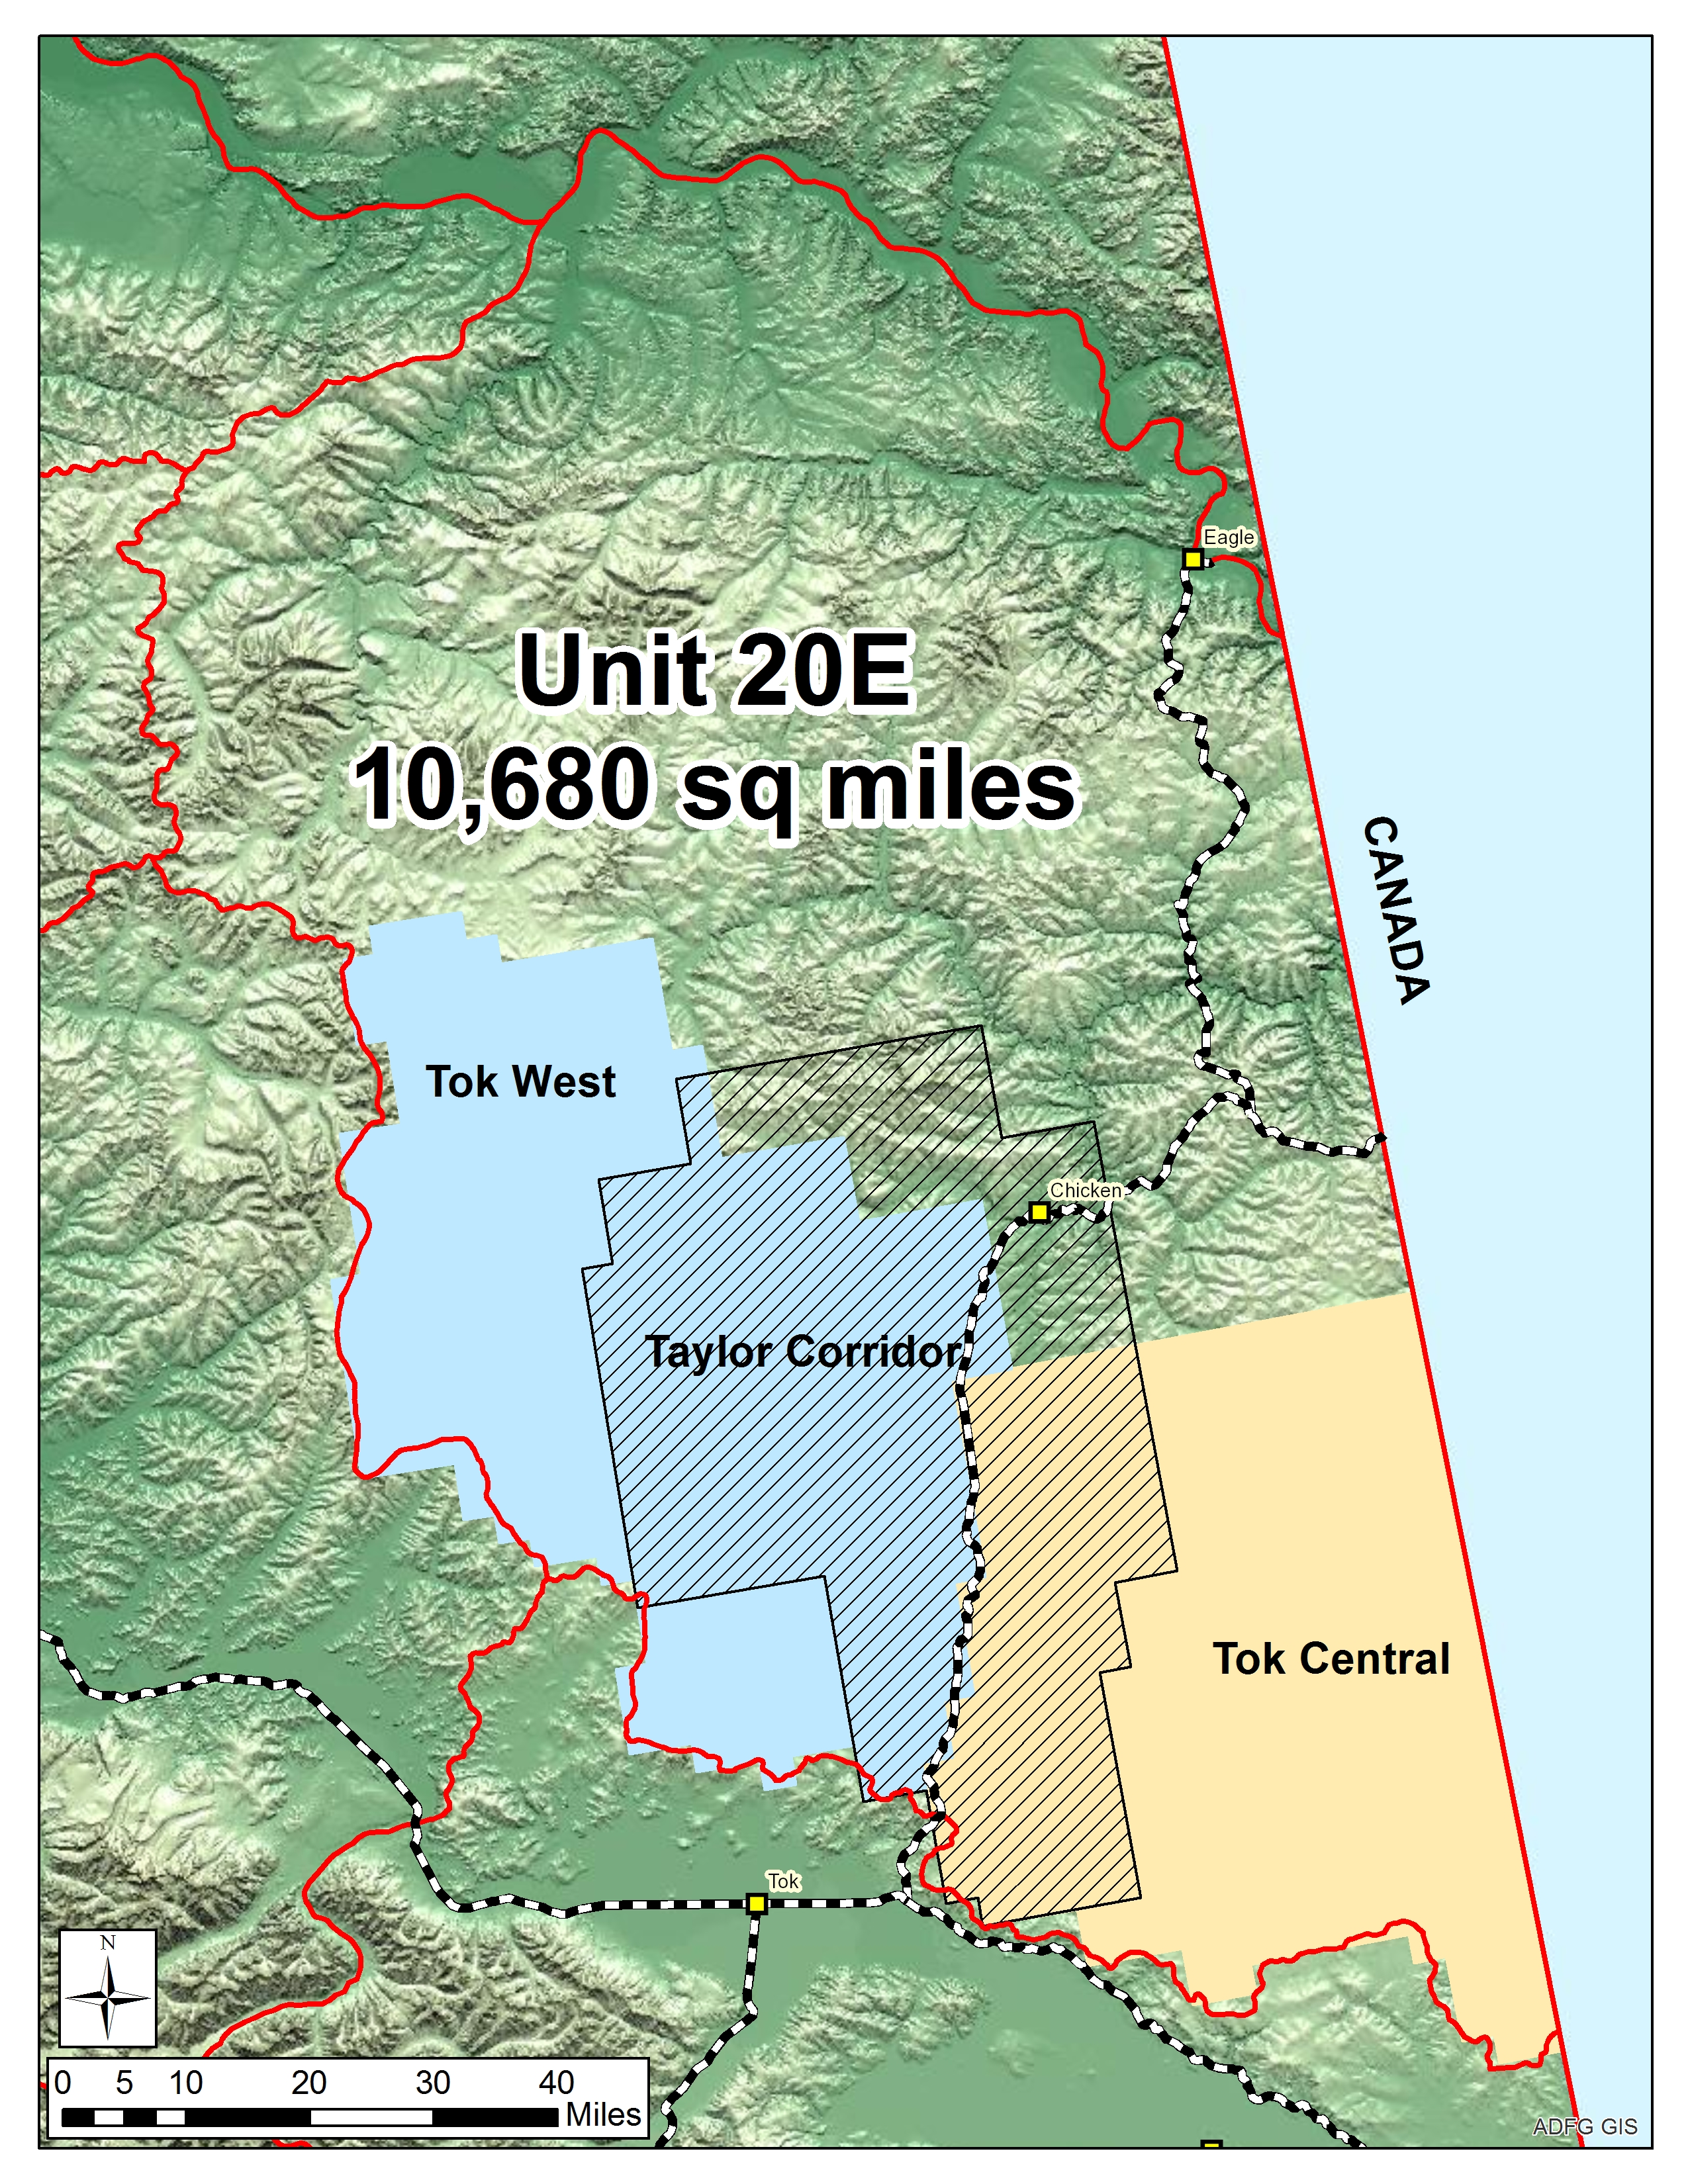
\includegraphics[width=0.5\linewidth]{20E_survey_area_overview} \caption{\label{fig:tokplot} A map of the Taylor Corridor in the Tok region of Alaska.}\label{fig:unnamed-chunk-2}
\end{figure}

The Taylor Corridor in the Tok region of Alaska is a popular habitat for
moose and other wildlife. Abundance surveys for moose are performed in
the Taylor Corridor of the Tok region of Alaska annually (Figure
\ref{fig:tokplot}) so that biologists have an idea about the abundance
of moose each year. In particular, surveys were conducted every year
from 2014 through 2020 in every year except 2016, during which there was
not sufficient snow cover to perform a survey. The spatial sampling
frame for one particular survey consists of 381 sites. There are a total
of 7 unique time points represented in the data, including the missing
year of 2016. Therefore, \(N\) is 2667.

In each year of the survey, an aerial team of biologists selects some of
the 381 sites to survey. The number of sites that are selected varies
from a low of 76 in the year 2019 to a high of 90 in the year 2020.
Throughout the 7 unique years, some sites are sampled as many as five
different times while others are never sampled at all (Figure
\ref{fig:tokplotyears}). The number of units sampled throughout all
survey years, \(n\), is 487 units.

\begin{figure}
\centering
\includegraphics{fpspatiotemp_manu_files/figure-latex/tokplotyears-1.pdf}
\caption{\label{fig:tokplotyears} Layout of the spatial sites used to
survey moose in the Taylor corridor of the TOK region of Alaska,
coloured by moose count. The year 2016 is excluded because no survey was
performed in that year. This and all remaining figure graphics are
constructed with the \texttt{ggplot2 R} package \citep{wickham2016data}}
\end{figure}

Before the survey begins in each year, biologists stratify the sites
into a \texttt{"HIGH"} stratum composed of 230 sites and a
\texttt{"LOW"} stratum composed of 151 sites. The goal of the following
analysis is to predict the total abundance of moose across all sites in
the year \texttt{2020}, the most recent year of the survey, using
stratum as a covariate in the spatio-temporal model.

\subsection{Model Fitting} \label{subsection:modelfit}

We fit the product-sum covariance model defined in equation
\ref{equation:model} using REML with stratum as a covariate in the
design matrix, an exponential spatial correlation structure defined in
equation \ref{equation:spatcov}, and an exponential temporal correlation
structure defined in equation \ref{equation:tempcov}. Table
\ref{tab:paramest} gives the estimated parameters from the model fit.

\begin{table}[H]

\caption{\label{tab:paramest}Estimated covariance parameters in the model. $\hat{\sigma}^2_{\delta}$, $\hat{\sigma}^2_{\gamma}$, and $\hat{\phi}$ are the spatial dependent error variance, independent error variance, and range parameters, respectively. $\hat{\sigma}^2_{\tau}$, $\hat{\sigma}^2_{\eta}$, and $\hat{\rho}$ are the temporal dependent error variance, independent error variance, and range parameters, respectively. $\hat{\sigma}^2_{\omega}$ and $\hat{\sigma}^2_{\nu}$ are the spatio-temporal dependent error variance and spatio-temporal independent error variance.}
\centering
\begin{tabular}[t]{cccccccc}
\toprule
\multicolumn{3}{c}{Spatial} & \multicolumn{3}{c}{Temporal} & \multicolumn{2}{c}{Spatio-temporal} \\
\cmidrule(l{3pt}r{3pt}){1-3} \cmidrule(l{3pt}r{3pt}){4-6} \cmidrule(l{3pt}r{3pt}){7-8}
$\hat{\sigma}^2_{\delta}$ & $\hat{\sigma}^2_{\gamma}$ & $\hat{\phi}$ & $\hat{\sigma}^2_{\tau}$ & $\hat{\sigma}^2_{\eta}$ & $\hat{\rho}$ & $\hat{\sigma}^2_{\omega}$ & $\hat{\sigma}^2_{\nu}$\\
\midrule
16.91 & 3.76 & 4.44 & 0.88 & 0.25 & 2.29 & 24.01 & 30.8\\
\bottomrule
\end{tabular}
\end{table}

To help interpret what some of these fitted covariance parameter
estimates mean, we can construct a fitted covariance plot (Figure
\ref{fig:covplot}). As the spatial distance between two sites increases
(dark colour to light colour), the covariance of two errors decreases to
0, with the \(\hat{\phi}\) parameter estimate controlling the rate of
decay. In fact, the model estimates the covariance to be nearly 0 when
two sites are 20 or more units apart, no matter what the temporal
distance is. The covariance between two errors that are six years apart
is still estimated to be positive if the two errors come from the same
site or from adjacent sites.

\begin{figure}
\centering
\includegraphics{fpspatiotemp_manu_files/figure-latex/covplot-1.pdf}
\caption{\label{fig:covplot} Estimated covariance of the errors from the
estimated parameters in a spatio-temporal product-sum model. The
centroids of two sites directly adjacent to one another are about 4
units apart.}
\end{figure}

The estimated vector of fixed effects, using \texttt{"HIGH"} as the
reference group, is \(\bm{\hat{\beta}}\) = (11.26, -9.76). Therefore,
the overall mean for sites in the \texttt{"HIGH"} stratum is estimated
to be 11.26 moose while the overall mean for sites in the \texttt{"LOW"}
stratum is estimated to be 1.5 moose.

\subsection{Prediction}

We now use the fitted spatio-temporal model with the BLUP from equation
\ref{equation:blup} and weights given in equation
\ref{equation:currentweights} to predict the total abundance across all
sites in the year 2020, the most recent year of the survey. Plugging in
estimates of the covariance parameters into equations
\ref{equation:blup} and \ref{equation:predvar} and letting elements of
\(\mathbf{b}_a\) be equal to 1 for data points in 2020 and equal to 0
otherwise, we obtain a prediction of 2874 moose and a standard error
(the square root of the prediction variance) of 234 moose. A 90\%
normal-based prediction interval for the total abundance in 2020 is
(2489, 3259) moose. Note that, though the response in this example is a
count, a normal-based prediction interval for the total is still
appropriate through an application of the central limit theorem for
dependent data \citep{smith1980central}. Sitewise predictions for sites
in 2020 are given in the map in Figure \ref{fig:sitepredmap}.

\begin{figure}
\centering
\includegraphics{fpspatiotemp_manu_files/figure-latex/unnamed-chunk-9-1.pdf}
\caption{\label{fig:sitepredmap} A map of the predictions for the sites
in the year 2020. A site with a grey dot in the center means that the
site was sampled in 2020.}
\end{figure}

For comparison, we use the spatial \texttt{sptotal} package
\citep{higham2021sptotal} to compute the spatial FPBK prediction
\citep{ver2008spatial} for the total abundance of moose in the year 2020
with stratum as a covariate. The spatial FPBK predictor is what is
currently implemented in the widely used GSPE software for moose surveys
\citep{delong2006geospatial}.

We also use the stratified random sampling design-based estimator
\mbox{} \begin{equation*}
\sum_{i = 1}^{2} N_i \cdot \bar{y}_i
\end{equation*} \noindent where \(\bar{y}_i\) is the sample mean for the
observed data in 2020 in the \(i^{th}\) stratum and \(N_i\) is the total
number of sites in 2020 in the \(i^{th}\) stratum. The stratified random
sampling design-based estimator has a variance for the total abundance
of \mbox{} \begin{equation*}
\sum_{i = 1}^{2} N_i^2 \cdot (1 - \frac{n_i}{N_i}) \cdot \frac{s^2_i}{n_i},
\end{equation*} \noindent where \(s^2_i\) is the sample variance of the
observed data points in 2020 in the \(i^{th}\) stratum and \(n_i\) is
the number of observed data points in 2020 in the \(i^{th}\) stratum.
Both the purely spatial model fit with \texttt{sptotal} and the
stratified random sampling design-based estimator use data only from
2020.

For the purely spatial model, the prediction for the total number of
moose in 2020 in the region is 2870 moose with a standard error of 319
moose. For the stratified random sampling design-based estimator, the
estimated total number of moose in 2020 in the region is 2853 moose with
a standard error of 371 moose. While the predictions for the total moose
abundance are somewhat similar across the three methods, we see that the
spatio-temporal model is most efficient (\(SE\) = 234 moose compared to
319 moose for the purely spatial model that ignores previous surveys and
371 moose for the stratified random sampling design-based estimator that
ignores both previous surveys and spatial correlation in the current
survey).

\section{Simulation} \label{section:Simulation}

\subsection{Description}

To evaluate performance of the st-FPBK predictor, we conduct a
simulation study. We simulate a response vector \(\mathbf{y}\) of length
\(N = 1000\) on a \(10 \times 10\) grid of 100 spatial sites on the unit
square (\([0, 1] \times [0, 1]\)) and 10 equally-spaced time points in
the interval \([0, 1]\), so that each spatial site has a response value
at each time point. \(\mathbf{y}\) is multivariate normal with mean
\(\mathbf{0}\) and product-sum covariance matrix \(\bm{\Sigma}\) defined
in equation \ref{equation:var} with the covariance parameters given in
Table \ref{tab:simparmtab}.

\begin{table}[H]

\caption{\label{tab:simparmtab}Covariance parameters used to simulate data. $\sigma^2_{\delta}$, $\sigma^2_{\gamma}$, and $\phi$ are the spatial dependent error variance, independent error variance, and range parameters, respectively. $\sigma^2_{\tau}$, $\sigma^2_{\eta}$, and $\rho$ are the temporal dependent error variance, independent error variance, and range parameters, respectively. $\sigma^2_{\omega}$ and $\sigma^2_{\nu}$ are the spatio-temporal dependent error variance and spatio-temporal independent error variance.}
\centering
\begin{tabular}[t]{ccccccccc}
\toprule
\multicolumn{1}{c}{ } & \multicolumn{3}{c}{Spatial} & \multicolumn{3}{c}{Temporal} & \multicolumn{2}{c}{Spatio-temporal} \\
\cmidrule(l{3pt}r{3pt}){2-4} \cmidrule(l{3pt}r{3pt}){5-7} \cmidrule(l{3pt}r{3pt}){8-9}
scenario & $\sigma^2_{\delta}$ & $\sigma^2_{\gamma}$ & $\phi$ & $\sigma^2_{\tau}$ & $\sigma^2_{\eta}$ & $\rho$ & $\sigma^2_{\omega}$ & $\sigma^2_{\nu}$\\
\midrule
all-dev & 0.5 & 0.17 & 0.47 & 0.5 & 0.17 & 0.33 & 0.50 & 0.17\\
t-iev & 0 & 0 & 0.47 & 0 & 1.50 & 0 & 0.25 & 0.25\\
spt-iev & 0 & 0 & 0 & 0 & 0 & 0 & 0 & 2.00\\
\bottomrule
\end{tabular}
\end{table}

The three scenarios in the table correspond to (1) \textbf{all-dev}: a
scenario where a substantial proportion of the overall variance comes
from the spatial, temporal, and spatio-temporal dependent error variance
parameters \(\sigma^2_{\delta}, \sigma^2_{\tau},\) and
\(\sigma^2_{\omega}\); (2) \textbf{t-iev}: a scenario where there the
overall variance is dominated by the temporal independent error variance
parameter, \(\sigma^2_{\eta}\); and (3) \textbf{spt-iev}: a scenario
where all of the variability comes from \(\sigma^2_{\nu}\) so that
errors are independent regardless of spatial and time indices. In all
scenarios, summing all six variance parameters gives a total variance
equal to two units squared.

Both \(\mathbf{R}_{s}\) and \(\mathbf{R}_t\) are generated from the
exponential correlation function with \(\phi\) and \(\rho\) as the range
parameters in equations \ref{equation:spatcov} and
\ref{equation:tempcov}. The values \(0.471\) and \(0.3333\) are chosen
for \(\phi\) and \(\rho\), respectively, so that the effective ranges,
\(3 \phi\) and \(3 \rho\), are equal to the maximum distance between two
data points in space (\(\sqrt2 = 1.414\)) and the maximum distance
between two data points in time (\(1\)). A value of 0 for \(\phi\) (or
\(\rho\)) sets the \(\mathbf{R}_{s}\) (or the \(\mathbf{R}_t\)) matrix
to the identity matrix. Figure \ref{fig:simcovplot} shows the model
covariance of the errors used to generate data for the ``all-dev''
scenario.

\begin{figure}
\centering
\includegraphics{fpspatiotemp_manu_files/figure-latex/unnamed-chunk-27-1.pdf}
\caption{\label{fig:simcovplot} The model covariance used in the
simulations for the spatio-temporal scenario. Covariance is
approximately 0 for errors from data points that are \(\sqrt2\) distance
units apart in space or 1 distance unit apart in time. The spatial
dependent error variance (\(\sigma^2_{\delta}\)), spatial independent
error variance (\(\sigma^2_{\gamma}\)), temporal dependent error
variance (\(\sigma^2_{\tau}\)), and temporal independent error variance
(\(\sigma^2_{\eta}\)) are shown with grey lines.}
\end{figure}

Each of these three scenarios is replicated for two different sample
sizes: \(n = 250\) and \(n = 500\). A simple random sample of the 1000
total data points is used to select units to be in the sample.

Finally, the simulation experiment is repeated for a skewed response
variable. To create the skewed response variable, a normally-distributed
response is simulated according to the parameters given in Table
\ref{tab:simparmtab}, except that each of the variance parameters (not
including \(\phi\) and \(\rho\)) is divided by 2.89 so that the total
variance is equal to 0.6931. This variable is then exponentiated so that
the total variance after exponentiation is equal to 2. Note that, not
only does exponentiation result in a right-skewed response variable, but
exponentiating also allows for an assessment of how the st-FPBK
predictor performs when the covariance is mis-specified, as the
resulting response variable is now simulated with an intractable
covariance function form that is not used in the model fitting.

Therefore, the simulation study has \(12\) total settings coming from a
\(3 \times 2 \times 2\) (scenario \(\times\) sample size \(\times\)
distribution shape) factorial design. For each setting, we simulate 1000
realizations of the response vector \(\mathbf{y}\). For each
realization, we use three methods to predict the total response for the
``most current'' time point, which is when the time index is equal to 1
on the interval \([0, 1]\)). We will henceforth call this ``total
response for the most current time point quantity'' the ``current
total.''

The first method uses the st-FPBK predictor in equation
\ref{equation:blup} with the spatio-temporal model covariance in
equation \ref{equation:var}. REML estimation with the observed data
\(\mathbf{y}_o\) is used to obtain estimates for the covariance
parameter vector \(\bm{\theta}\). The second method is the FPBK spatial
model fit with the \texttt{sptotal R} package \citep{higham2021sptotal}
that only uses data from the most current time point.

The third method uses a simple random sample (SRS) design-based
estimator with data from the most current time point. The SRS
design-based estimator for the total is \(100 \cdot \bar{y}\), where
\(\bar{y}\) is the sample mean of the response in the most current time
point. The variance of the estimator \citep{lohr2021sampling} is
\(100^2 \cdot \frac{s^2}{n_1} \cdot (1 - \frac{n_1}{100})\), where
\(s^2\) is the sample variance of the response variable in the most
current time point and \(n_1\) is the number of sampled locations in the
most current time point.

The SRS method gives an estimator, not a predictor, and a corresponding
confidence interval, not a prediction interval, because the SRS
design-based estimator treats the observed data as fixed, not as a
random realization from a process
\citep{brus2021statistical, dumelle2022comparison}. However, in the
remaining text and tables, we refer to the ``current total'' response
quantity obtained from the three methods as a ``prediction'' and to the
corresponding interval as a ``prediction interval'' to limit
unnecessarily verbose text and tables.

For each method, we calculate the root-mean-squared-prediction-error
(rMSPE) as
\(\frac{1}{1000}\sqrt{(\sum_{i = 1}^{1000}(T_i - \hat{T}_i)^2)}\), where
\(T_i\) and \(\hat{T}_i\) are the realized and predicted current totals,
respectively, in the \(i^{th}\) iteration. Bias is recorded as
\(\frac{1}{1000}\sum_{i = 1}^{1000}(T_i - \hat{T}_i)\). We also create a
normal-based 90\% prediction interval for the realized current total and
record \(\frac{1}{1000} \sum_{i = 1}^{1000}I(LB_i < T_i < UB_i)\), where
\(I(LB_i < T_i < UB_i)\) is an indicator variable that is equal to \(1\)
if the realized total in iteration \(i\), \(T_i\), is between the lower
bound, \(LB_i\), and the upper bound, \(UB_i\), of the \(i^{th}\)
prediction interval.

\subsection{Results}

Tables \ref{tab:simrmspetab}, \ref{tab:simbiastab}, and
\ref{tab:simpitab} in Section \ref{section:appendix} give the rMSPE,
bias, and interval coverage of the three methods in all 12 simulation
settings. In Figure \ref{fig:rmspe}, we see that the st-FPBK predictor
outperforms both the purely spatial FPBK predictor and the simple random
sample design-based estimator in all of the ``all-dev'' and ``spt-iev''
scenarios. In general, rMSPE improvement is larger for the smaller
sample size.

We see little gains in rMSPE for the st-FPBK predictor in the ``t-iev''
scenario. This setting was chosen to explore how the spatio-temporal
model would perform when most of the variability in the response comes
from \(\sigma^2_{\eta}\), which allows for data collected in different
time points to be uncorrelated, and, for different time points to have
very different realized totals. As expected, the st-FPBK predictor
performs no better than a purely spatial model or the SRS design-based
estimator for this scenario; however, we can also say that the added
complexity of the spatio-temporal model is not detrimental.

\begin{figure}
\centering
\includegraphics{fpspatiotemp_manu_files/figure-latex/unnamed-chunk-29-1.pdf}
\caption{\label{fig:rmspe} root-mean-squared-prediction-error (rMSPE)
for all simulation settings. The st-FPBK predictor has the smallest
rMSPE in all settings tested, though it is similar to the rMSPE of the
other two methods in the t-iev scenario.}
\end{figure}

All methods appear relatively unbiased in all simulation settings: Table
\ref{tab:simbiastab} shows that the bias of each method is small
compared to the squares of the rMSPE values given in Table
\ref{tab:simrmspetab}.

Figure \ref{fig:pi} shows the interval coverage for the normal-based
prediction intervals \citep{smith1980central}, where the nominal level
is 0.90. We see that the st-FPBK predictor for the current total has
approximate 90\% coverage in all settings tested. The spatial model and
the SRS design-based estimator have lower than nominal coverage in some
settings because of the small sample size used (recall that the
\(n = 250\) observed samples span 10 unique time points so that, on
average, the spatial model and SRS design-based estimator only have 25
observed responses to use in the current time point).

\begin{figure}
\centering
\includegraphics{fpspatiotemp_manu_files/figure-latex/unnamed-chunk-30-1.pdf}
\caption{\label{fig:pi} Prediction interval coverage for all simulation
settings, where the prediction intervals are normal-based and the
nominal level is 0.90. The st-FPBK predictor has close to appropriate
coverage in all settings tested.}
\end{figure}

\section{Discussion} \label{section:Discussion}

We see in the moose application in Section \ref{section:Application}
that there is substantial reduction in the standard error of the
predictor for the total moose abundance in 2020 when incorporating data
from surveys in previous years. In the simulation study in
\ref{section:Simulation}, we find that the st-FPBK predictor has lower
rMSPE than the FPBK predictor from a purely spatial model and an SRS
design-based estimator in many settings. The st-FPBK predictor is less
beneficial when the temporal independent error variance contributes a
large proportion to the overall variance. Additionally, the st-FPBK
predictor maintains appropriate interval coverage in all settings
tested, even when the covariance for the errors is mis-specified.

An additional possible benefit of using the st-FPBK predictor compared
to a purely spatial FPBK predictor is the potential for forecasting
abundance before a survey is completed. For example, in our application,
we can refit the model without any of the observed counts from the 2020
survey and examine the prediction for the total abundance in the year
2020. Table \ref{tab:forecast} compares the model with the 2020 data
used and the model without the 2020 data used. We see that, while there
is a substantial loss in precision by excluding the 2020 data (as we
would expect), the prediction is not very different from the prediction
with the 2020 data included. And, the prediction interval might be
narrow enough to still be useful to wildlife management. We could also
consider using such an approach if there is a year during which a survey
cannot be completed for logistical reasons. For example, in the Tok
region of Alaska, a moose survey was not conducted at all in the year
2016 because there was insufficient snow cover for the survey. The
spatio-temporal predictor could still be applied to get a prediction for
moose abundance using survey data from previous years.

\begin{table}[H]

\caption{\label{tab:forecast}Results from analysis on the Tok moose survey data with the 2020 survey included and excluded. We can see that, even with 2020 data excluded, we can obtain a prediction for moose abundance in 2020, though there is substantial loss in precision.}
\centering
\begin{tabular}[t]{lcccc}
\toprule
  & Prediction & SE & 90\% LB & 90\% UB\\
\midrule
2020 Data Included & 2874 & 234 & 2489 & 3259\\
2020 Data Excluded & 2757 & 417 & 2071 & 3444\\
\bottomrule
\end{tabular}
\end{table}

We would also like to give our perception of the benefits and drawbacks
of our approach with that of \citet{schmidt2022bayesian}, who use a
hierarchical Bayesian model to predict total abundance, among other
quantities of interest. The benefits of our frequentist approach include
a faster fitting time, as there is no need to construct and implement
the time-consuming Markov chain Monte Carlo sampler. Therefore, our
approach is easier to assess in a simulation study, which would be too
time-prohibitive for the Bayesian model. Biometricians could also use
simulation with our approach to answer various questions given proposed
values of covariance parameters like how much efficiency would drop if a
survey was only conducted every other year. Additionally, we argue that
our approach is simpler overall for a practitioner to use and could be
integrated more readily with the current GSPE software.

The Bayesian approach by \citet{schmidt2022bayesian}, however, offers
features that would be harder to implement in our approach. In general,
the model is more flexible, and allows for incorporation of more levels
in the Bayesian hierarchical model, including allowing for imperfect
detection of animals from a separate detectability survey. Additionally,
the Bayesian hierarchical model can use a Poisson or negative binomial
model for the counts. Therefore, an appropriate prediction interval for
the response on one particular site could be constructed. On the other
hand, for our approach, we rely on the central limit theorem for
dependent data to form a prediction interval for the total, which would
not apply for a prediction interval for the response on just one site.

We have developed a finite population block kriging predictor for
spatio-temporal data, which adjusts the variance of the predictor to be
appropriate for sampling from a finite population. In many settings, the
resulting predictor is improved from a predictor with a purely spatial
model. Monitoring programs that use regularly scheduled surveys should
consider incorporating data from past surveys to improve precision in
the predictor for the most current survey.

Future work in this area includes developing a frequentist model for
which imperfect detection of units through time is incorporated into the
predictor or how best to select sites to sample for future surveys given
proposed values for the spatio-temporal covariance parameters.
Additionally, for moose surveys in particular, updating the GSPE
software to include analysis for spatio-temporal data could be useful
for practitioners. Though we recognize that doing so would be a
substantial undertaking, the \texttt{R} package that we provide could be
a useful starting point for the integration.

\section{Appendix} \label{section:appendix}

\begin{table}[H]

\caption{\label{tab:simrmspetab}root-mean-squared-prediction-error (rMSPE) for the st-FPBK predictor, the FPBK predictor, and the SRS estimator for each of the 12 simulation settings. In all settings, the rMSPE for the st-FPBK predictor is approximately equal to or lower than the rMSPE for the other two methods.}
\centering
\begin{tabular}[t]{cccccc}
\toprule
\multicolumn{3}{c}{Simulation Setting} & \multicolumn{3}{c}{rMSPE} \\
\cmidrule(l{3pt}r{3pt}){1-3} \cmidrule(l{3pt}r{3pt}){4-6}
scenario & n & Response Type & st-FPBK & FPBK & SRS\\
\midrule
spt-iev & 250 & normal & 14.58 & 25.06 & 24.64\\
t-iev & 250 & normal & 10.31 & 10.53 & 10.76\\
all-dev & 250 & normal & 11.18 & 14.97 & 17.23\\
\midrule
spt-iev & 500 & normal & 10.84 & 14.91 & 14.71\\
t-iev & 500 & normal & 6.12 & 6.22 & 6.50\\
all-dev & 500 & normal & 6.09 & 8.43 & 10.24\\
\midrule
spt-iev & 250 & lognormal & 15.49 & 26.14 & 24.56\\
t-iev & 250 & lognormal & 11.89 & 12.10 & 12.05\\
all-dev & 250 & lognormal & 14.28 & 18.35 & 19.46\\
\midrule
spt-iev & 500 & lognormal & 11.22 & 15.38 & 15.04\\
t-iev & 500 & lognormal & 7.34 & 7.32 & 7.82\\
all-dev & 500 & lognormal & 7.55 & 9.89 & 11.45\\
\bottomrule
\end{tabular}
\end{table}

\begin{table}[H]

\caption{\label{tab:simbiastab}Bias (Realized Current Total - Predicted Current Total) for the st-FPBK predictor, the FPBK predictor, and the SRS estimator for each of the 12 simulation settings. In all settings, all methods appear fairly unbiased.}
\centering
\begin{tabular}[t]{cccccc}
\toprule
\multicolumn{3}{c}{Simulation Setting} & \multicolumn{3}{c}{Bias} \\
\cmidrule(l{3pt}r{3pt}){1-3} \cmidrule(l{3pt}r{3pt}){4-6}
scenario & n & Response Type & st-FPBK & FPBK & SRS\\
\midrule
spt-iev & 250 & normal & 0.73 & 1.38 & 1.55\\
t-iev & 250 & normal & 0.44 & 0.39 & 0.47\\
all-dev & 250 & normal & 0.48 & 0.27 & 0.45\\
\midrule
spt-iev & 500 & normal & 0.46 & 0.60 & 0.67\\
t-iev & 500 & normal & 0.15 & 0.14 & 0.07\\
all-dev & 500 & normal & 0.04 & 0.07 & 0.04\\
\midrule
spt-iev & 250 & lognormal & 0.36 & 0.56 & 1.48\\
t-iev & 250 & lognormal & 0.33 & 0.22 & 0.41\\
all-dev & 250 & lognormal & -0.07 & -0.85 & -0.49\\
\midrule
spt-iev & 500 & lognormal & 0.32 & 0.29 & 0.66\\
t-iev & 500 & lognormal & 0.24 & 0.15 & 0.08\\
all-dev & 500 & lognormal & -0.10 & -0.39 & -0.37\\
\bottomrule
\end{tabular}
\end{table}

\begin{table}[H]

\caption{\label{tab:simpitab}Prediction interval coverage for the st-FPBK predictor, the FPBK predictor, and the SRS for each of the 12 simulation settings. All intervals are normal-based and have a nominal coverage level of 0.90.}
\centering
\begin{tabular}[t]{cccccc}
\toprule
\multicolumn{3}{c}{Simulation Setting} & \multicolumn{3}{c}{Coverage} \\
\cmidrule(l{3pt}r{3pt}){1-3} \cmidrule(l{3pt}r{3pt}){4-6}
scenario & n & Response Type & st-FPBK & FPBK & SRS\\
\midrule
spt-iev & 250 & normal & 0.92 & 0.87 & 0.89\\
t-iev & 250 & normal & 0.91 & 0.88 & 0.91\\
all-dev & 250 & normal & 0.90 & 0.88 & 0.91\\
\midrule
spt-iev & 500 & normal & 0.90 & 0.86 & 0.88\\
t-iev & 500 & normal & 0.89 & 0.87 & 0.89\\
all-dev & 500 & normal & 0.88 & 0.89 & 0.89\\
\midrule
spt-iev & 250 & lognormal & 0.90 & 0.82 & 0.84\\
t-iev & 250 & lognormal & 0.90 & 0.86 & 0.90\\
all-dev & 250 & lognormal & 0.89 & 0.86 & 0.89\\
\midrule
spt-iev & 500 & lognormal & 0.89 & 0.84 & 0.84\\
t-iev & 500 & lognormal & 0.89 & 0.87 & 0.88\\
all-dev & 500 & lognormal & 0.89 & 0.87 & 0.89\\
\bottomrule
\end{tabular}
\end{table}

\bibliographystyle{tfcad}
\bibliography{interactcadsample.bib}





\end{document}
